\documentclass{article}
\usepackage[utf8]{inputenc}
\usepackage[english, russian]{babel}
\usepackage{graphicx}
\graphicspath{ {./graphics/} }
\usepackage[a4paper, total={6in, 8in}]{geometry}
\pagestyle{empty} %
\usepackage[pageanchor]{hyperref}
\usepackage{enumitem}
\usepackage{listings}
\usepackage{amssymb}
\usepackage{amsmath}
\usepackage{indentfirst}
\usepackage{tikz}

\newcommand{\kaucher}{
  \begin{tikzpicture}
    \draw (0, 0) circle (0.6ex);
    \draw (-0.6ex, 0) -- (0.6ex, 0);
  \end{tikzpicture}%
}

\begin{document}
  \begin{titlepage}
    \begin{center}
      Санкт-Петербургский политехнический университет \\Петра Великого
    \end{center}

    \begin{center}
      Физико-механический институт
    \end{center}

    \begin{center}
      Высшая школа прикладной математики и вычислительной\\ физики
    \end{center}

    \vspace{8em}

    \begin{center}
      \textbf{Отчет по лабораторной работе №3}\\
      \textbf{“Интервальный анализ”}
    \end{center}

    \vspace{\fill}

    \begin{flushright}
      \noindentВыполнили студент группы 5030102/10201:
      \hfill
      Скворцов Владимир Сергеевич \\
    \end{flushright}
    Преподаватель: \hfill Баженов Александр Николаевич

    \vspace{12em}

    \begin{center}
      Санкт-Петербург\\
      2024
    \end{center}
  \end{titlepage}

  \tableofcontents

  \newpage

  \section{Постановка задачи}

  Даны 2 интервальных выборки

  \begin{equation}
    \mathbf{X} = \{ \mathbf{x}_i \},
  \end{equation}
  \begin{equation}
    \mathbf{Y} = \{ \mathbf{y}_i \}.
  \end{equation}

  Взять \( \mathbf{X}, \mathbf{Y} \) из файлов данных, задав
  \( \text{rad} \mathbf{x} = \text{rad} \mathbf{y} = \frac{1}{2^N} \text{В} \),
  \( N = 14 \).

  Файлы данных:
  \begin{itemize}
    \item \emph{-0.205\_lvl\_side\_a\_fast\_data.bin}
    \item \emph{0.225\_lvl\_side\_a\_fast\_data.bin}
  \end{itemize}

  Связь кодов данных и В:

  \begin{equation*}
    V = N  / 16384 - 0.5
  \end{equation*}

  Сделать оценки констант \( a \), \( t \) в уравнениях:
  \begin{equation}
    \mathbf{X} + a = \mathbf{Y},
  \end{equation}
  \begin{equation}
    t\mathbf{X} = \mathbf{Y},
  \end{equation}

  Метод решения:

  \begin{equation}
    \hat a = \text{argmax} F(a, \mathbf{X}, \mathbf{Y}),
  \end{equation}

  где \( F \) --- функционал.

  В качестве функционала взять варианты:

  \begin{equation} \label{eq:F_1}
    \text{Ji} (a, \mathbf{X}, \mathbf{Y}),
  \end{equation}
  \begin{equation} \label{eq:F_2}
    \text{Ji} (a, \text{mode} \mathbf{X}, \text{mode} \mathbf{Y}),
  \end{equation}
  \begin{equation} \label{eq:F_3}
    \text{Ji} (a, \text{med}_K \mathbf{X}, \text{med}_K \mathbf{Y}),
  \end{equation}
  \begin{equation} \label{eq:F_4}
    \text{Ji} (a, \text{med}_P \mathbf{X}, \text{med}_P \mathbf{Y}),
  \end{equation}

  где \( \text{Ji} \) --- коэффициент Жаккара,
  \( \text{mode} \) --- интервальная мода,
  \( \text{med}_K \), \( \text{med}_P \) --- интервальные медианы Крейновича
  и Пролубникова.

  Сделать точечные и интервальные оценки, задавшись уровнем \( \alpha \).

  \section{Необходимая теория}

  \subsection{Интервальная мода}

  Пусть имеется интервальная выборка

  \[
    \mathbf{X} = \{ \mathbf{x}_i \}.
  \]

  Сформируем массив интервалов \( \mathbf{z} \) из концов интервалов
  \( \mathbf{X} \).

  Для каждого интервала \( \mathbf{z}_i \) подсчитываем число \( \mu_i \)
  интервалов из выборки \( \mathbf{X}_i \), включающих \( \mathbf{z}_i \).
  Максимальные \( \mu_i = \max \mu \) достигаются для индексного множества
  \( K \). Тогда можно найти интервальную моду как мультиинтервал

  \begin{equation}
    \text{mode} \mathbf{X} = \bigcup_{k \in K} \mathbf{z}_k.
  \end{equation}

  \subsection{Интервальная медиана Крейновича}

  Пусть дана выборка \( \mathbf{X} = \{ \mathbf{x}_i \} \). Пусть
  \( \underline c = \{ \underline{\mathbf{x}_i} \} \),
  \( \overline c = \{ \overline{\mathbf{x}_i} \} \) --- конфигурация
  точек, составленные, соответственно, из левых и правых концов интервалов
  из \( \mathbf{X} \).

  Тогда медианой Крейновича \( \text{med}_K \mathbf{X} \) интервальной
  выборки \( \mathbf{X} \) --- это интервал

  \begin{equation}
    \text{med}_K = [\text{med} \underline c, \text{med} \overline c].
  \end{equation}

  \subsection{Интервальная медиана Пролубникова}

  Зададим отношение порядка на алгебре \( \mathbb{IR} \). Говорят, что
  неравенство \( \mathbf{a} \leqslant \mathbf{b} \) выполняется

  \begin{enumerate}
    \item в сильном смысле, если
      \( \forall \mathbf{a} \in \mathbb{IR} \ \forall \mathbf{b} \in \mathbb{IR}: \overline{\mathbf{a}} \leqslant \underline{\mathbf{b}} \),
    \item в слабом смысле, если
      \( \exists \mathbf{a} \in \mathbb{IR} \ \exists \mathbf{b} \in \mathbb{IR}: \underline{\mathbf{a}} \leqslant \overline{\mathbf{b}} \),
    \item в \( \forall \exists \)-смысле, если
      \( \forall \mathbf{a} \in \mathbb{IR} \ \exists \mathbf{b} \in \mathbb{IR}: \overline{\mathbf{a}} \leqslant \overline{\mathbf{b}} \),
    \item в \( \exists \forall \)-смысле, если
      \( \exists \mathbf{a} \in \mathbb{IR} \ \forall \mathbf{b} \in \mathbb{IR}: \underline{\mathbf{a}} \leqslant \underline{\mathbf{b}} \),
    \item в центральном смысле, если
      \( (\overline{\mathbf{a}} + \underline{\mathbf{a}}) / 2 \leqslant (\overline{\mathbf{b}} + \underline{\mathbf{b}}) / 2 \)
  \end{enumerate}

  Для элементов выборки \( \mathbf{X} \) можно определить линейный порядок,
  используя любое из пяти вышеуказанных отношений порядка на
  \( \mathbb{IR} \). То есть, если \( i \ne j \), то либо
  \( x_i \leqslant x_j \), либо \( x_i \geqslant x_j \) для любого из
  этих отношений порядка.

  Медиана Пролубникова \( \text{med}_P \mathbf{X} \) выборки
  \( \mathbf{X} \) --- это интервал \( \mathbf{x}_m \), для которого
  половина интервалов из \( \mathbf{X} \) лежит слева, а половина
  --- справа.

  В ситуации, когда имеются два элемента подинтервала \( \mathbf{x}_m \)
  и \( \mathbf{x}_{m+1} \), распо­ложенных посередине вариационного ряда,
  \( \mathbf{x}_m \ne \mathbf{x}_{m+1} \) медиана может быть определена
  естественным обобщением взятия полусуммы точечных значений,
  расположенных посередине ряда из точечных значений, в случае
  интервальной выборки взятие полусуммы интервалов \( \mathbf{x}_m \)
  и \( \mathbf{x}_{m+1} \):

  \begin{equation}
    \text{med}_P \mathbf{X} = (\mathbf{x}_m + \mathbf{x}_{m+1}) / 2.
  \end{equation}

  \subsection{Коэффициент Жаккара}

  Коэффициент Жаккара для двух интервалов \( \mathbf{x} \in \mathbb{IR} \)
  и \( \mathbf{y} \in \mathbb{IR} \):

  \begin{equation}
    \text{Ji} (\mathbf{x}, \mathbf{y})
      = \frac{\text{wid} (x \land y)}{\text{wid} (x \lor y)}
      = \frac{\min \{ \overline{\mathbf{x}}, \overline{\mathbf{y}} \} - \max \{ \underline{\mathbf{x}}, \underline{\mathbf{y}} \}}
        {\max\{ \overline{\mathbf{x}}, \overline{\mathbf{y}} \} - \min \{ \underline{\mathbf{x}}, \underline{\mathbf{y}} \}}.
  \end{equation}

  Коэффициент Жаккара для множества интервалов
  \( \mathbf{X} \in \mathbb{IR}^n \):

  \begin{equation}
    \text{Ji} (\mathbf{X})
      = \frac{\min \overline{\mathbf{x}_i} - \max \underline{\mathbf{x}_i}}
        {\max \overline{\mathbf{x}_i} - \min \underline{\mathbf{x}_i}}.
  \end{equation}

  Коэффициент Жаккара для двух множеств интервалов
  \( \mathbf{X} \in \mathbb{IR}^n \) и \( \mathbf{Y} \in \mathbb{IR}^n \):

  \begin{equation}
    \text{Ji}_k (\mathbf{X}, \mathbf{Y})
      = \frac{\min \{ \overline{\mathbf{x}_k}, \overline{\mathbf{y}_k} \} - \max \{ \underline{\mathbf{x}_k}, \underline{\mathbf{y}_k} \}}
        {\max\{ \overline{\mathbf{x}_k}, \overline{\mathbf{y}_k} \} - \min \{ \underline{\mathbf{x}_k}, \underline{\mathbf{y}_k} \}},
      \ k \in 1, 2, \dots, |\mathbf{X}|.
  \end{equation}

  \section{Реализаця}

  Лабораторная работа выполнена на языке программирования Python. В ходе
  работы были также использованы библиотеки \verb!numpy! и
  \verb!matplotlib!.

  Ссылка на GitHub репозиторий:
  \href{https://github.com/vladimir-skvortsov/spbstu-interval-anylysis}
  {https://github.com/vladimir-skvortsov/spbstu-interval-anylysis}

  \subsection{Поиск параметров, при которых функционал достигал наибольших
  значений}

  Для поиска параметров, при которых функционал достигал наибольших
  значений, был использован алгоритм троичного поиска с заданной точностью
  \( \varepsilon = 10^{-3} \) на участках, где функции вели
  себя как унимодальные.

  \section{Результаты}

  \begin{figure}[htbp!]
		\begin{center}
			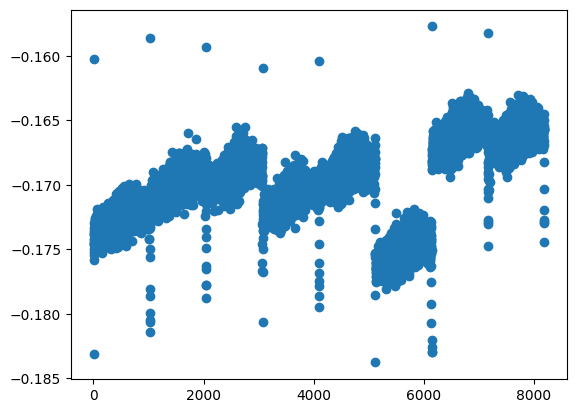
\includegraphics[width = 0.45\textwidth]{x_mean.png}
			\caption{Усредненные данные в выборке X}
      \label{figure:int_est}
		\end{center}
  \end{figure}

  \begin{figure}[htbp!]
		\begin{center}
			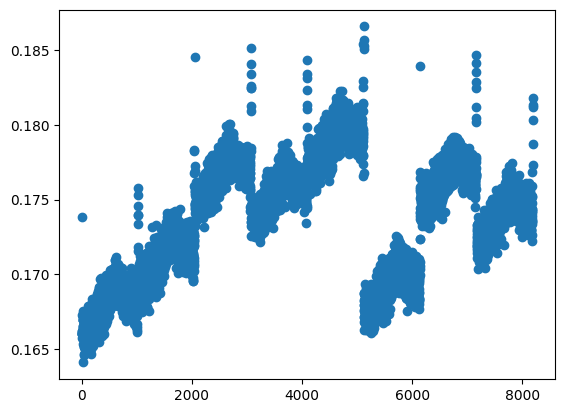
\includegraphics[width = 0.45\textwidth]{y_mean.png}
			\caption{Усредненные данные в выборке Y}
      \label{figure:int_est}
		\end{center}
  \end{figure}

  \clearpage

  Для функцинала \ref{eq:F_1}:

  \[ \hat a = 0.34601 \pm 0.0005, \ F_1 (\hat a) = -0.94918, \]
  \[ \hat t = -1.05038 \pm 0.0005, \ F_1 (\hat t) = -0.92734. \]

  Для функцинала \ref{eq:F_2}:

  \[ \hat a = 0.34675 \pm 0.0005, \ F_2 (\hat a) = -0.25437, \]
  \[ \hat t = -1.03947 \pm 0.0005, \ F_2 (\hat t) = -0.92750. \]

  Для функцинала \ref{eq:F_3}:

  \[ \hat a = 0.34406 \pm 0.0005, \ F_3 (\hat a) = -0.00184, \]
  \[ \hat t = -1.02773 \pm 0.0005, \ F_3 (\hat t) = 0.63020. \]

  Для функцинала \ref{eq:F_4}:

  \[ \hat a = 0.34406 \pm 0.0005, \ F_4 (\hat a) = -0.12457, \]
  \[ \hat t = -1.02773 \pm 0.0005, \ F_4 (\hat t) = 0.63021. \]

  \section{Выводы}

  В ходе выполнения лабораторной работы были изучены методы оценки
  параметров в уравнениях с интервальными данными. Используя различные
  функционалы, такие как коэффициент Жаккара, были найдены оптимальные
  значения параметров \( \hat a \) и \( \hat t \) для уравнений
  \( \mathbf{X} + a = \mathbf{Y} \) и \( t\mathbf{X} = \mathbf{Y} \).

  Результаты показали, что:

  \begin{enumerate}
    \item Значения параметров \( \hat a \) и \( \hat t \) варьируются в
      зависимости от выбранного функционала. Это демонстрирует важность
      выбора подходящего критерия оптимальности для конкретной задачи
      интервального анализа.
    \item Наиболее стабильные результаты были получены для функционала
      \ref{eq:F_3}, где значение \( \hat t \) показало положительное
      значение коэффициента Жаккара, что указывает на высокий уровень
      совпадения интервалов.
    \item Выбор интервальной моды и медиан (Крейновича и Пролубникова) как
      статистических характеристик позволил получить более точные оценки
      параметров, что подчеркивает их значимость в анализе интервальных
      данных.
  \end{enumerate}

  Таким образом, проведенная работа продемонстрировала применимость и
  эффективность интервального анализа в задачах оценки параметров, а также
  подчеркнула важность выбора подходящих методов и инструментов для
  анализа данных.
\end{document}
